% $Id: configurator.tex,v 1.1 2003/10/01 20:36:37 naughtont Exp $
%
% "Configurator HOWTO" (LaTeX-ified for inclusion w/ the Pkg howto)
%  - The details the usage and syntax for working with the OSCAR Configurator.
%


\section{OSCAR Configurator}
\label{sect:configurator}

This section provides details on the syntax and usage of the OSCAR
Configurator. 

\subsubsection*{Writing the \file{configurator.html} File}

To present configuration options to the user, the Configurator uses
a simple HTML \textbf{Form}. While the basics of writing HTML files
and HTML forms are discussed in detail in many books and online tutorials,
this section seeks to describe the HTML form tags available to a package
maintainer and how to use those tags to get information from the user.

Many of the basic HTML tags are supported in the OSCAR Configurator,
including:

\begin{itemize}
\item various fonts and headers 
\item line and paragraph breaks 
\item horizontal (ruler) lines 
\item centered text 
\item images (GIFs and JPEGs) 
\end{itemize}
There is also a decent assortment of HTML Form tags such as:

\begin{itemize}
\item input fields
\item checkboxes
\item radio buttons
\item single- and multi-selection lists
\item text boxes 
\end{itemize}
All of the available tags are described in detail below.

There are some HTML tags that are NOT allowed in a configuration file.
In particular, you may \textbf{not} use:

\begin{itemize}
\item $<$A HREF$>$ - A hypertext link to other places on the web. We don't want
the user going off to another web page.
\item $<$TABLE$>$, $<$TR$>$, $<$TD$>$ - While tables are parsed in without difficulty,
they are not rendered as true talbes. Better to use $<$PRE$>$ (preformatted
text) for this purpose.
\item $<$ISINDEX$>$ - The document cannot be searchable.
\item Form $<$SUBMIT$>$, $<$BUTTON$>$, and $<$IMAGE$>$ - The Configurator has its own
button to submit the values of the form to the program, so these elements
are unnecessary.
\item $<$FILE$>$ - The user is not allowed to upload a file. 
\end{itemize}
If any of these tags are present in your HTML document, they are removed
prior to rendering so that your document will appear without the offending
tags.


\subsubsection*{A Basic HTML Form Document}

Since all of the configuration input from a user appears in an HTML
Form, the minimum useful configuration file contains $<$form$>$ and
$<$/form$>$
tags. Between these two tags, the package maintainer adds $<$input$>$
tags to get input from the user. For example, if all you want from
the user is his name, your configuration file might be as follows:

\begin{footnotesize}
\begin{verbatim}
     <form>
     Enter your name: <input name="username">
     </form>
\end{verbatim}
\end{footnotesize}

The resulting output would look like this:


% \begin{figure}[h!]
%   \begin{center}
%     
\includegraphics[scale=\imgscale]{figs/EnterYourName}
%     %\caption{}
%     \label{fig:config-enter-name}
%   \end{center}
% \end{figure}

~


\includegraphics[%
  %scale=0.5]{EnterYourName.png}
  scale=0.5]{figs/EnterYourName}

~


If you are HTML savvy, you may notice a few things missing from this
example. Specifically, we omitted the main $<$html$>$...$<$/html$>$ tags,
and the $<$head$>$$<$/head$>$ and $<$body$>$$<$/body$>$ tags. For basic configuration
files, these tags are optional. You may use them if you like (and
some browsers would bonk if they were absent), but they are not required.
Also, there are no attributes for the $<$form$>$ tag. This is because
the Configurator knows the action to take when the user saves the
values, so no {}``action'' label is needed. Also, there can be only
one pair of $<$form$>$$<$/form$>$ tags in the configuration file, so there
is no need for the {}``name'' label.


\subsubsection*{A More Complete HTML Form}

A typical HTML document consists of at least two separate sections,
a {}``head'' and a {}``body''. The most important element of the
{}``head'' is the $<$title$>$...$<$/title$>$ tag. This sets the title of
the window and also acts as the text for the header of the configuration
window. If you omit this tag or leave the value blank, it defaults
to {}``Configuration''.

The body is where the main part of the HTML document is stored. It
includes both the Form and any other {}``standard'' HTML elements
you want to display. Many of these elements can appear inside or outside
of the Form, so it is sometimes easiest to have a configuration form
that looks like this:

\begin{footnotesize}
\begin{verbatim}
     <html>
       <head>
         <title>The Title Of Your Configuration Form<title>
       </head>

       <body> 
         <form> 
           All of your main HTML configuration goes here.
         </form> 
       </body> 
     </html>
\end{verbatim}
\end{footnotesize}

In HTML files, whitespace (including carriage returns) are usually
compacted to a single space. So in the above example, the indentation
and line spacing are shown simply to make the example easier to read.
We could just have easily put everything on a single line and the
output would be the same. This is important to know since if you want
a true line break (say between paragraphs), you have to explicitly
tell HTML by using the $<$p$>$ (paragraph) tag. Also, the case of the
tags is unimportant, so you could also use all uppercase letters for
your tags if you find that to be more readable.


\subsubsection*{Basic (non-form) HTML Tags}

There are many HTML tags which can be displayed by the Configurator
that don't need to be in the form, but will be useful anyway. The
function of each of these tags are not listed here. There are plenty
of HTML reference books and online tutorials available. Use your favorite
search engine and do a search on {}``HTML tutorial'' to get a big
listing.


\subsubsection*{HTML Form Tags}

The main tags that you will need for your configuration file are $<$form$>$
tags. These tags allow you to prompt the user for information to be
entered via text boxes, check boxes, radio buttons, selection lists,
etc. This section describes each tag in detail and provides examples.

Note that all of these tags must appear between a $<$form$>$...$<$/form$>$
tag pair. Otherwise your values will not get submitted correctly.

\begin{itemize}
\item $<$input type=\char`\"{}text\char`\"{} name=\char`\"{}VARIABLE\char`\"{}
value=\char`\"{}INITIAL\char`\"{} size=\char`\"{}NUMCHARS\char`\"{}
maxlength=\char`\"{}MAXCHARS\char`\"{}$>$ - 


A \textit{text} element is a single line text input field in which
the user can enter text. If you do not specify \textbf{type=''text''},
then the $<$input$>$ defaults to this type of text input field. Of the
various attributes, only \textbf{name} is required. The \textbf{name}
attribute designates the variable name for the data entered by the
user. If you also specify the \textbf{value} attribute, that text
appears in the text input field when it first appears. The \textbf{size}
and \textbf{maxlength} attributes designate the number of characters
that appear in the text box and the maximum length of the input text
respectively.

Example:

\begin{footnotesize}
\begin{verbatim}
     <form> 
     Enter your name: 
     <input type="text" name="username" value="johndoe" size="20" maxlength="30"> 
     </form>
\end{verbatim}
\end{footnotesize}

Output:

%%TJN: NEW need new capture
%\begin{figure}[h!]
%  \begin{center}
%    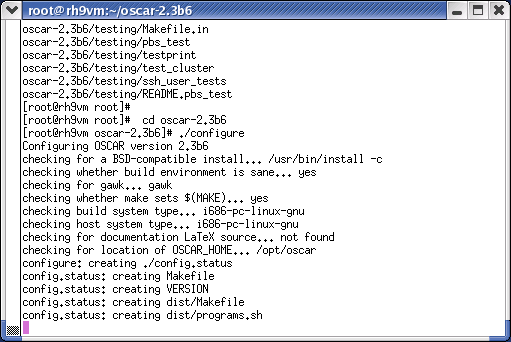
\includegraphics[scale=\imgscale]{figs/sbs-configure-install}
%    %\caption{}
%    \label{fig:config-enter-name2}
%  \end{center}
%\end{figure}


\begin{quote}

\includegraphics[%
  %scale=0.5]{EnterYourName2.png}
  scale=0.5]{figs/EnterYourName2}
\end{quote}
\item $<$input type=\char`\"{}password\char`\"{} name=\char`\"{}VARIABLE\char`\"{}
value=\char`\"{}INITIAL\char`\"{} size=\char`\"{}NUMCHARS\char`\"{}
maxlength=\char`\"{}MAXCHARS\char`\"{}$>$ -


A \textit{password} element is a text input field in which each character
typed is displayed as a {*} to conceal the actual value entered. In
all other aspects, this element is the same as the \textit{text} element.

Example:

\begin{footnotesize}
\begin{verbatim}
     <form> 
     Enter your password: 
     <input type="password" name="password" value="passwd" size="10" maxlength="20"> 
     </form>
\end{verbatim}
\end{footnotesize}

Output: 

\begin{quote}

\includegraphics[%
  %scale=0.5]{EnterYourPassword.png}
  scale=0.5]{figs/EnterYourPassword.eps}
\end{quote}
\item $<$input type=\char`\"{}checkbox\char`\"{} name=\char`\"{}VARIABLE\char`\"{}
value=\char`\"{}RETURNVALUE\char`\"{} checked$>$ - 


A \textit{checkbox} is a toggle that the user can select (switch on)
or deselect (switch off). As with all $<$input$>$ elements, the \textbf{name}
attribute is required and designates the variable name for the value
returned by the check box. Usually, {}``ON'' is returned when a
check box has been checked by the user. If you specify the \textbf{value}
attribute, that value is returned instead when the check box has been
checked by the user. You can optionally specify the \textbf{checked}
attribute to make the check box initially selected when first displayed.
Otherwise, the check box is unselected when first displayed. Any check
boxes which are not checked when the form is submitted do not get
passed to the Configurator, ie. their values will be {}``'' (the
empty string).

Example:

\begin{footnotesize}
\begin{verbatim}
     <form> 
     <input type="checkbox" name="rootaccess" value="YES" checked> 
     Enable "root" access 
     </form>
\end{verbatim}
\end{footnotesize}

Output: 

\begin{quote}

\includegraphics[%
  %scale=0.5]{EnableRootAccess.png}
  scale=0.5]{figs/EnableRootAccess.eps}
\end{quote}
\item $<$input type=\char`\"{}radio\char`\"{} name=\char`\"{}VARIABLE\char`\"{}
value=\char`\"{}RETURNVALUE\char`\"{} checked$>$ - 


A \textit{radio} element is a radio button. A set of radio buttons
consists of multiple radio buttons that all have the same \textbf{name}
attribute. Only one radio button in the set can be selected at one
time. When the user selects a button in the set, all other buttons
in the set are deselected. If one radio button in a set has the \textbf{checked}
attribute, that one is selected when the set is first displayed. Otherwise,
none of the radio buttons are selected when first displayed (which
may not be the desired functionality). As with all $<$input$>$ elements,
the \textbf{name} attribute is required and designates the variable
name for the value returned by the radio button set. All radio buttons
with the same \textbf{name} are in the same set, regardless of where
they appear in the form. The \textbf{value} attribute is the value
that is returned for the radio button set when the form is submitted.
This default to {}``ON'' which isn't very useful for a set of radio
buttons, so be sure to give each radio button its own \textbf{value}.

Example:

\begin{footnotesize}
\begin{verbatim}
     <form> 
     User type:<br> 
     <input type="radio" name="usertype" value="guest"> Guest<br> 
     <input type="radio" name="usertype" value="user" checked> User<br> 
     <input type="radio" name="usertype" value="admin"> Admin<br> 
     </form>
\end{verbatim}
\end{footnotesize}

Output: 

\begin{quote}
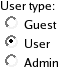
\includegraphics[%
  %scale=0.5]{UserType.png}
  scale=0.5]{figs/UserType}
\end{quote}
\item $<$input type=\char`\"{}hidden\char`\"{} name=\char`\"{}VARIABLE\char`\"{}
value=\char`\"{}RETURNVALUE\char`\"{}$>$ - 


A \textit{hidden} element is an invisible element whose main purpose
is to contain data that the user does not enter. This data gets sent
when the form is submitted. This allows you to always pass a certain
name/value pair to the Configurator without input from the user. Both
the \textbf{name} and \textbf{value} attributes are required.

Example:

\begin{footnotesize}
\begin{verbatim}
     <form> 
     There's a hidden element here!
     <input type="hidden" name="version" value="5.23"> 
     </form>
\end{verbatim}
\end{footnotesize}

Output: 

\begin{quote}

\includegraphics[%
  %scale=0.5]{HiddenElement.png}
  scale=0.5]{figs/HiddenElement}
\end{quote}
\item $<$input type=\char`\"{}reset\char`\"{}
value=\char`\"{}LABEL\char`\"{}$>$
- 


When the user presses a \textit{reset} button, all elements in the
form are reset to the values that were present when the form was first
displayed. Usually, the text of this button is {}``Reset'', but
you can change this by specifying the \textbf{value} attribute.

Example:

\begin{footnotesize}
\begin{verbatim}
     <form> 
     Reset form: <input type="reset" value="Reset to Original Values">
     </form>
\end{verbatim}
\end{footnotesize}

Output: 

\begin{quote}

\includegraphics[%
  %scale=0.5]{ResetForm.png}
  scale=0.5]{figs/ResetForm}
\end{quote}
\item $<$textarea name=\char`\"{}VARIABLE\char`\"{} cols=\char`\"{}WIDTH\char`\"{}
rows=\char`\"{}HEIGHT\char`\"{} 


wrap=\char`\"{}OFF\char`\"{}|\char`\"{}HARD\char`\"{}|\char`\"{}SOFT\char`\"{}$>$Text
to display$<$/textarea$>$ - 

The \textit{textarea} tag defines a multiline input field into which
the user can enter text. As with $<$input$>$ elements, the \textbf{name}
attribute is required and designates the variable name for the text
present in the box when the form is submitted. The width and height
(in terms of characters) of the text box is given by the optional
\textbf{cols} and \textbf{rows} attributes. By default, any text entered
by the user is displayed {}``as is'' meaning that if the line input
by the user is longer than the width of the text box, the text will
scroll off the screen. The only time a new row is started is when
the user types a carriage return. This is also the behavior when you
use the \textbf{wrap=\char`\"{}OFF\char`\"{}} attribute. If you want
to have the text word wrap automatically, use the \textbf{wrap=\char`\"{}HARD\char`\"{}}
or \textbf{wrap=\char`\"{}SOFT\char`\"{}} attribute. (In standard
HTML, these two attributes differ by whether or not the extra carriage
returns generated by word wrapping get submitted in the text or not.
For the Configurator, these extra carriage returns are never submitted,
which is equivalent to \textbf{wrap=\char`\"{}SOFT\char`\"{}}, so
using \textbf{wrap=\char`\"{}HARD\char`\"{}} generates the same behavior.)
Between the two $<$textarea$>$...$<$/textarea$>$ tags, you can put optional
{}``Text to display'' when the textarea is first displayed.

Example:

\begin{footnotesize}
\begin{verbatim}
     <form> 
     Comments?<br> 
     <textarea name="comments" cols=40 rows=5 wrap="SOFT"> 
     Enter your comments or suggestions here. 
     </textarea> 
     </form>
\end{verbatim}
\end{footnotesize}

Output: 

\begin{quote}
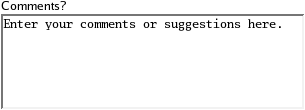
\includegraphics[%
  %scale=0.5]{Comments.png}
  scale=0.5]{figs/Comments}
\end{quote}
\item $<$select name=\char`\"{}VARIABLE\char`\"{} size=\char`\"{}LISTLENGTH\char`\"{}
multiple$>$ $<$option value=\char`\"{}OPTIONVALUE\char`\"{}$>$ $<$option value=\char`\"{}OPTIONVALUE\char`\"{}
selected$>$ ... $<$/select$>$ - 


The \textit{select} and \textit{option} tags define a selection list.
A selection list displays a list of options from which the user can
select one (or more) items. If the \textbf{multiple} attribute is
present, the user can select multiple items from the list at a time.
Otherwise, only a single item can be selected at a time. As with \textbf{input}
elements, the \textbf{name} attribute is required and designates the
variable name for the value(s) selected in the list when the form
is submitted. The optional \textbf{size} attribute indicates how many
items are presented in the box before scrolling is necessary. This
defaults to {}``10''. If you set \textbf{size} to {}``1'' and
do not set the \textbf{multiple} attribute, you get a single element
drop-down list.

To actually put items in the selection list, you use the \textit{option}
tag followed by the text you wish to appear in the list. You can make
that option selected when the list is initially displayed by using
the \textbf{selected} attribute. By default, the value that gets returned
to the Configurator when an item is selected is the actual text of
the item in the list. You can override this behavior by using the
optional \textbf{value} attribute. When you set this value, it gets
returned when that item in the list is selected.

Example:

\begin{footnotesize}
\begin{verbatim}
     <form> 
     Select the machines to use:<br> 
     <select name="machinelist" size=5 multiple> 
     <option selected>oscar1 
     <option>oscar2 
     <option>oscar3 
     <option>oscar4 
     <option>oscar5 
     <option>oscar6 
     <option value="unlisted">unlisted machine 
     </select> 
     </form>
\end{verbatim}
\end{footnotesize}

Output: 

\begin{quote}
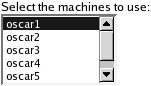
\includegraphics[%
  %scale=0.5]{SelectMachine.png}
  scale=0.5]{figs/SelectMachine}
\end{quote}
Note: when viewing the above example in a standard HTML browser, you
might have to use the $<$SHIFT$>$ or $<$CTRL$>$ key in conjunction with clicking
the mouse to select multiple items from the list. In the Configurator,
this extra keypress is not required.\end{itemize}

